\section{Auswertung}
\subsection{Ablenkung im elektrischen Feld}
Es werden die Messdaten Strahlablenkung $D$, Plattenspannung $U_d$ und die Beschleunigungsspannung $U_B$ notiert.
Sie sind in der Tabelle \ref{tab:1} dargestellt.
\begin{table}[H]
  \centering
  \caption{Die Messwerte der Parameters.}
  \label{tab:1}
  \begin{tabular}{c c c c c c}
\toprule
& \multicolumn{1}{c}{$U_B=\SI{200}{\volt}$} & \multicolumn{1}{c}{$U_B=\SI{250}{\volt}$} &\multicolumn{1}{c}{$U_B=\SI{300}{\volt}$}&\multicolumn{1}{c}{$U_B=\SI{400}{\volt}$}&\multicolumn{1}{c}{$U_B=\SI{500}{\volt}$}\\
\cmidrule(lr){2-2}\cmidrule(lr){3-3}\cmidrule(lr){4-4}\cmidrule(lr){5-5}\cmidrule(lr){6-6}
$D \, / \, cm$ & $U_d \, / \, V$ & $U_d \, / \, V$ & $U_d \, / \, V$ &$U_d \, / \, V$ & $U_d \, / \, V$\\
\midrule
5.080 & 21,9  & 28,9  & 33,8  & -    & -   \\
4.445 & 19,1  & 24,6  & 29,0  & -    & -   \\
3.810 & 14,9  & 19,6  & 23,3  & 30,7 & -   \\
3.175 & 11,2  & 14,6  & 17,2  & 22,9 & 31,3\\
2.540 &  6,5  &  8,5  & 10,2  & 14,7 & 21,2\\
1.905 &  2,5  &  4,5  &  4,7  &  6,1 & 10,2\\
1.270 & -1,6  & -0,7  & -1,6  & -1,0 & -0,5\\
0.635 & -5,3  & -5,9  & -7,4  & -9,2 &-11,3\\
0.000 & -9,3  &-10,6  &-13,9  &-17,0 &-21,6\\
\bottomrule
  \end{tabular}
\end{table}
Nun werden die Parameter $D$ und $U_d$ gegeneinander aufgetragen.
Dies ist in der Abbildung \ref{abb:6} dargestellt.
\begin{figure}[H]
  \centering
  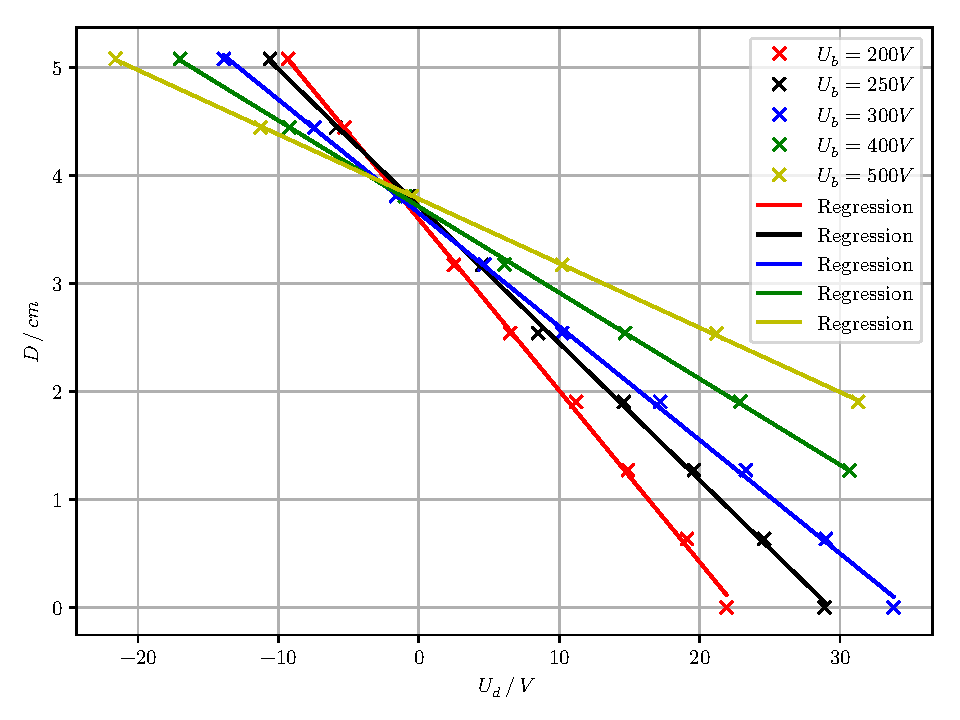
\includegraphics{plot1.pdf}
  \caption{Darstellung der Messdaten.}
  \label{abb:6}
\end{figure}
Die lineare Ausgleichsrechnung wurde mit Python 3.6 durchgeführt.
Dazu wurde die Gleichung \ref{eq:1} verwendet:
\begin{equation*}
  \underbrace{D}_{\mathclap{y}} = \underbrace{\frac{pL}{2dU_B}}_{\mathclap{m}} \cdot \underbrace{U_d}_{\mathclap{x}} + b
\end{equation*}
Die folgenden Steigungen $m_{1-5}$ sind in der Tabelle \ref{tab:2} dargestellt.

\begin{table}[H]
  \centering
  \caption{Ergebnis der Ausgleichsrechnung.}
  \label{tab:2}
  \begin{tabular}{c c c}
\toprule
&$\text{Steigung} \,/\, \si{\centi\meter\per\volt}$& $U_B \, /\, \si{\volt}$\\
\midrule
$m_1$ & $\num{0.1587(22)}$& 200\\
$m_2$ & $\num{0.1268(13)}$& 250\\
$m_3$ & $\num{0.1051(12)}$& 300\\
$m_4$ & $\num{0.0797(6)}$ & 400\\
$m_5$ & $\num{0.0596(3)}$ & 500\\
\bottomrule
  \end{tabular}
\end{table}
Nun werden die Steigungen, in diesem Fall die Empfindlichkeiten $\frac{D}{U_d}$, gegen $\frac{1}{U_B}$ aufgetragen.
Die Darstellung ist in Abbildung \ref{abb:7} zu sehen.
\begin{figure}[H]
  \centering
  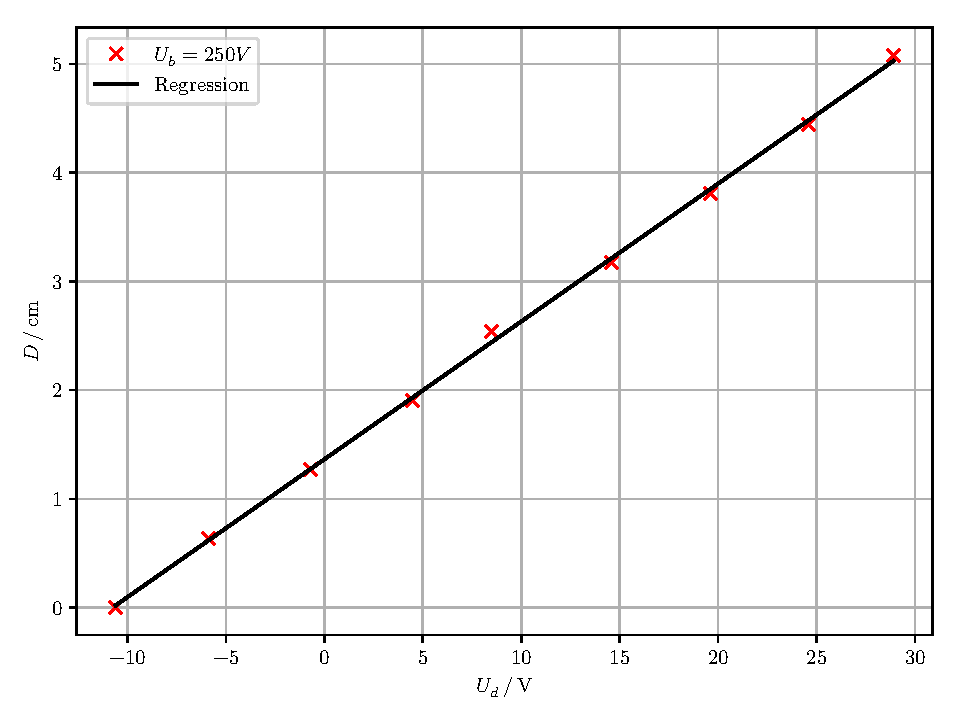
\includegraphics[width=\textwidth]{plot2.pdf}
  \caption{Darstellung zur Bestimmung der Konstruktionskonstante $a$.}
  \label{abb:7}
\end{figure}
Auch hier wurde eine lineare Ausgleichsrechnung mit Python 3.6 durchgeführt.
Dazu wurde die Gleichung \ref{eq:1} erneut verwendet:
\begin{equation*}
  \underbrace{\frac{D}{U_d}}_{\mathclap{y}} = \underbrace{\frac{pL}{2d}}_{\mathclap{a}} \cdot \underbrace{\frac{1}{U_B}}_{\mathclap{x}} + b
\end{equation*}
Es folgt somit für die Konstruktionskonstante $a$
\begin{equation*}
  a = \SI{32,59(72)}{\centi\meter}.
\end{equation*}
Der theoretische Wert kann mithilfe der Abbildung \ref{abb:5} selbst errechnet werden.
Dabei ist
\begin{itemize}
  \item $p = \SI{1.9}{\centi\meter}$
  \item $L = \SI{14.3}{\centi\meter}$
  \item $d = \SI{0.38}{\centi\meter}$
\end{itemize}
Es folgt somit für die Konstruktionskonstante
\begin{equation*}
  a_{\text{Theo}} = \frac{pL}{2d} = \SI{35.75}{\centi\meter}
\end{equation*}
Es entspricht einer Abweichung von $8,84 \%$ vom gemessenen Wert.\\
\newline
Es soll nun die Frequenz der Sinusspannung mithilfe der Sägezahnspannung
berechnet werden.
Dazu wird die Gleichung \ref{eq:2} genutzt. Dabei ist $m = 1$ und der
Proportionalitätsfaktor $n= 0.5, 1, 2, 3$
Die Messwerte werden in die Gleichung \ref{eq:2} eingesetzt und berechnet.
Die Ergebnisse sind in der Tabelle \ref{tab:3} dargestellt.
\begin{table}[H]
  \centering
  \caption{Ergebnisse zur Bestimmung der Sinusspannung.}
  \label{tab:3}
  \begin{tabular}{c c c}
\toprule
$\nu_{Sä} \,/\, \si{\hertz}$& $\text{Proportionalitätsfaktor} n$ & $\nu_{Si} \, /\, \si{\hertz}$\\
\midrule
29,33 & 3 & 87,99\\
49,99 & 2 & 99,98\\
79,32 & 1 & 79,32\\
158,64& 0,5& 79,32\\
\bottomrule
  \end{tabular}
\end{table}
Die Ergebnisse werden nun gemittelt.
Für den Mittelwert sowie die Standardabweichung werden die Formeln \ref{fel:1} und \ref{fel:2}
\begin{equation}
    \bar{\nu}_{Si}= \frac{1}{N} \sum_{i=1}^{N} \nu_{Si,i}
    \label{fel:1}
\end{equation}

\begin{equation}
  \Delta \bar{\nu}_{Si} = \frac{1}{\sqrt{N}\sqrt{N-1}} \sqrt{\sum_{i}(\nu_{Si,i}-\bar{\nu}_{si})^2}
  \label{fel:2}
\end{equation}
verwendet.
Es folgt für die Frequenz der Sinusspannung:
\begin{equation*}
  \nu_{si}= \SI{86.65(488)}{\hertz}
\end{equation*}
Des Weiteren soll der Scheitelwert mithilfe der Strahlablenkung $D$ und der Konstruktionskonstante $a$ berechnet werden.
Es wurde eine Beschleunigungsspannung $U_b = \SI{300}{\volt}$ angelegt. Die gemessene Konstruktionskonstante ist
$a = \SI{32,59(72)}{\centi\meter}$.
Bei den Messungen ergab sich konstant eine Strahlablenkung von $D = \SI{3.81}{\centi\meter}$.
Nun kann die Gleichung \ref{eq:1} umgeformt werden nach  der Plattenspannung $U_d$.
Es folgt:
\begin{equation*}
  U_d = \frac{D U_B}{a} = \SI{35.1(8)}{\volt}
\end{equation*}
Der Fehler lässt sich mithilfe der Gaußfehlerfortpflanzung wie gefolgt aufschreiben
\begin{equation}
  \Delta U_d = \sqrt{\Bigl(-\frac{DU_B}{a^2}\cdot \Delta a\Bigr)^2}
\end{equation}
\subsection{Auslenkung im magnetischen Feld}
Um die spezifische Ladung der Elektronen bestimmen zu können, werden zunächst
die Messwerte der Ablenkung $D$, den Strom $I$, der durch die Helmholzspule geht, sowie die
Beschleunigungsspannung $U_B$ notiert.
Die Ergebnisse sind in der Tabelle \ref{tab:4} dargestellt.
\begin{table}[H]
  \centering
  \caption{Darstellung der Messergebnisse.}
  \label{tab:4}
  \begin{tabular}{c c c c c c}
\toprule
& \multicolumn{1}{c}{$U_B=\SI{200}{\volt}$} & \multicolumn{1}{c}{$U_B=\SI{250}{\volt}$} &\multicolumn{1}{c}{$U_B=\SI{300}{\volt}$}&\multicolumn{1}{c}{$U_B=\SI{400}{\volt}$}&\multicolumn{1}{c}{$U_B=\SI{500}{\volt}$}\\
\cmidrule(lr){2-2}\cmidrule(lr){3-3}\cmidrule(lr){4-4}\cmidrule(lr){5-5}\cmidrule(lr){6-6}
$D \, / \, cm$ & $I \, / \, A$ & $I \, / \, A$ & $I \, / \, A$ &$I \, / \, A$ & $I \, / \, A$\\
\midrule
0,635 & 0,30  & 0,30 & 0,40 & 0,40& 0,40\\
1,270 & 0,60  & 0,65 & 0,75 & 0,75& 0,80\\
1,905 & 0.95  & 1,00 & 1,15 & 1,15& 1,20\\
2,540 & 1,25  & 1,40 & 1,50 & 1,60& 1,65\\
3,175 & 1,60  & 1,62 & 1,90 & 2,00& 2,05\\
3,810 & 1,95  & 2,10 & 2,30 & 2,40& 2,50\\
4,445 & 2,25  & 2,50 & 2,70 & 2,85& 3,00\\
5,080 & 2,65  & 2,85 & 3,15 & 3,30& 3,40\\
\bottomrule
  \end{tabular}
\end{table}
Für das magnetische Feld $B$ wird die Gleichung \ref{eq:4} verwendet. Dabei ist die
Windungszahl $N = 20 $ und der Spulenradius $R = \SI{28.2}{\centi\meter}$.
Mit $\frac{D}{L^2+D^2}$ für $L = \SI{17.5}{\centi\meter}$ werden die wichtigen
Ergebnisse in der Tabelle \ref{tab:5} dargestellt.
\begin{table}[H]
  \centering
  \caption{Darstellung der wichtigen Ergebnisse.}
  \label{tab:5}
  \begin{tabular}{c c c c c c}
\toprule
& \multicolumn{1}{c}{$U_B=\SI{200}{\volt}$} & \multicolumn{1}{c}{$U_B=\SI{250}{\volt}$} &\multicolumn{1}{c}{$U_B=\SI{300}{\volt}$}&\multicolumn{1}{c}{$U_B=\SI{400}{\volt}$}&\multicolumn{1}{c}{$U_B=\SI{500}{\volt}$}\\
\cmidrule(lr){2-2}\cmidrule(lr){3-3}\cmidrule(lr){4-4}\cmidrule(lr){5-5}\cmidrule(lr){6-6}
$\frac{D}{L^2+D^2} \, /\, \frac{1}{m}$ & $B \,/\, mT$ & $B \,/\, mT$ &$B \,/\, mT$ &$B \,/\, mT$ &$B \,/\, mT$\\
\midrule
0,31 & 0,01913 & 0,01913 & 0,02551 & 0,02551 & 0,02551\\
0,62 & 0,03826 & 0,04145 & 0,04783 & 0,04783 & 0,05102\\
0,92 & 0,06058 & 0,06377 & 0,07334 & 0,07334 & 0,07653\\
1,20 & 0,07971 & 0,08928 & 0,09566 & 0,10203 & 0,10522\\
1,48 & 0,10203 & 0,10331 & 0,12117 & 0,12754 & 0,13073\\
1,74 & 0,12117 & 0,13392 & 0,14667 & 0,15305 & 0,15943\\
1,98 & 0,14349 & 0,15943 & 0,17218 & 0,18175 & 0,19131\\
2,21 & 0,16899 & 0,18175 & 0,20088 & 0,21045 & 0,21682\\
\bottomrule
  \end{tabular}
\end{table}
Nun werden die Daten aus der Tabelle \ref{tab:5} gegeneinander aufgetragen und
in der Abbildung \ref{abb:8} graphisch dargestellt.
\begin{figure}[H]
  \centering
  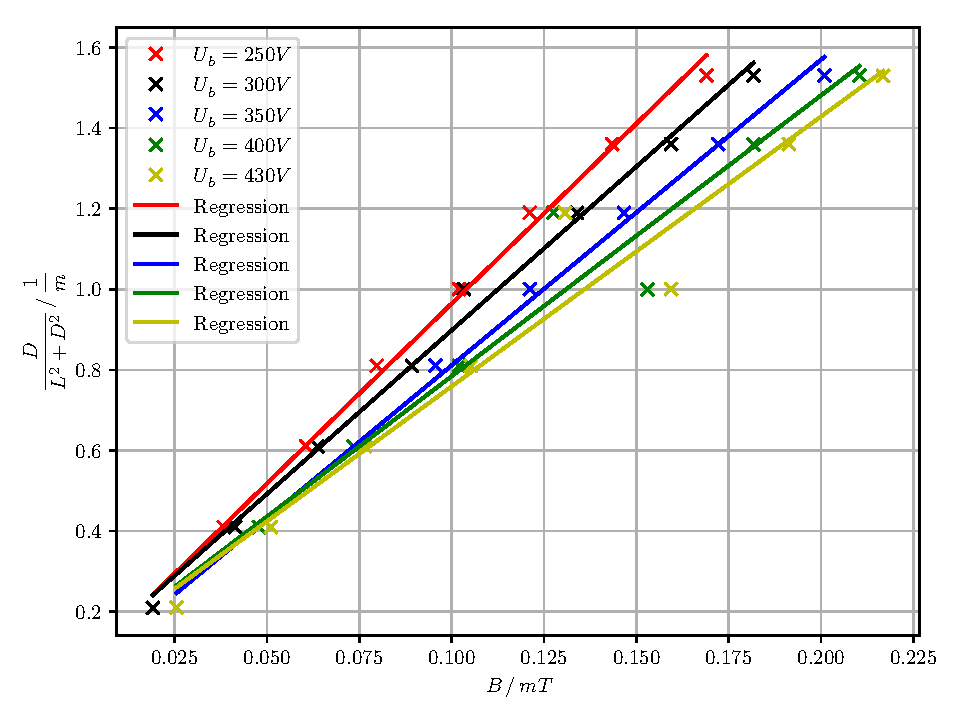
\includegraphics[width=\textwidth]{plot3.pdf}
  \caption{Darstellung der Messergebnisse.}
  \label{abb:7}
\end{figure}
Mit Python 3.6 wurde eine lineare Ausgleichsrechnung durchgeführt.
Dazu wurde die Gleichung \ref{eq:3} verwendet:
\begin{equation*}
  \underbrace{\frac{D}{L^2+D^2}}_{\mathclap{y}} = \underbrace{\frac{1}{\sqrt{8U_B}} \sqrt{\frac{e_0}{m_0}}}_{\mathclap{m}} \cdot \underbrace{B}_{\mathclap{x}} + b
\end{equation*}
Die Ergebnisse für die Bestimmung der spezifische Ladung $\frac{e_0}{m_0}$ werden
in der Tabelle \ref{tab:6} dargestellt. Dabei wurde folgende Rechnung angewendet
\begin{equation*}
  \frac{e_0}{m_0} = 8 \cdot U_B \cdot m_{1-5}^2
\end{equation*}
Der Fehler lässt sich mit der Gaußfehlerfortpflanzung bestimmen
\begin{equation*}
  \Delta \frac{e_0}{m_0} = \sqrt{(16 \cdot U_b \cdot m \cdot \Delta m)^2}.
\end{equation*}
Der theoretische Wert für die spezifische Ladung liegt bei:
\begin{equation*}
  \frac{e_0}{m_0}=\SI{1.76e11}{\coulomb\per\kilogram}
\end{equation*}

\begin{table}[H]
  \centering
  \caption{Darstellung der spezifische Ladung.}
  \label{tab:6}
  \begin{tabular}{c c c c}
\toprule
$\text{Beschleunigungsspannung}\, U_B \,/\, V$ & $\text{Steigung m} \,/\, \frac{1}{m\cdot mT}$ &$\frac{e_0}{m_0} \,/\, 10^{11}\frac{C}{kg}$ & $\text{Abweichung} \,/\, \%$\\
\midrule
250 &$\num{8.93(23)}$ &$\num{1.59(8)}$ &  9,66\\
300 &$\num{8.12(25)}$ &$\num{1.58(10)}$& 10,23\\
350 &$\num{7.58(19)}$ &$\num{1.61(8)}$ &  8,52\\
400 &$\num{6.97(64)}$ &$\num{1.55(29)}$& 11,93\\
430 &$\num{6.69(64)}$ &$\num{1.54(30)}$& 12,50\\
\bottomrule
  \end{tabular}
\end{table}

Zuletzt soll die Totalintensität des Erdmagnetfeldes errechnet werden.
Aus dem Spulenstrom kann das Magnetfeld, was in der Helmholzspule erzeugt wird,
berechnet werden.
Mit einem gemessenen Spulenstrom von
\begin{equation*}
  I_H =\SI{126}{\milli\ampere}
\end{equation*}
folgt mit Gleichung \ref{eq:4} für die Magnetfeldstärke:
\begin{equation*}
  B_H =\SI{8.035}{\micro\tesla}.
\end{equation*}
Zu beachten ist, dass die Magnetfeldstärke $B_H$ die horizontale Komponente es Erdmagnetfelds ist.
Wichtig hierbei ist unter welchem Winkel sich das Erdmagnetfeld ausrichtet.
Die gemessenen Winkeln zwischen Erdmagnetfeld und der Magnetfeldstärke in horizontale Komponente
sind in der Tabelle \ref{tab:7} dargestellt.
\begin{table}[H]
  \centering
  \caption{Messung des Winkels an verschiedenen Stellen.}
  \label{tab:7}
  \begin{tabular}{c}
\toprule
$\text{Winkel}\, \Phi \,/\, \circ$\\
\midrule
82\\
73\\
55\\
55\\
\bottomrule
  \end{tabular}
\end{table}
Mit Gleichung \ref{fel:1} und \ref{fel:2} wird der Mittelwert sowie die Standardabweichung berechnet.
\begin{equation*}
  \bar{\Phi}= \frac{1}{N} \sum_{i=1}^{N} \Phi_{i}
\end{equation*}
\begin{equation*}
\Delta \bar{\Phi} = \frac{1}{\sqrt{N}\sqrt{N-1}} \sqrt{\sum_{i}(\Phi_{i}-\bar{\Phi})^2}
\end{equation*}
Es folgt somit für den Winkel:
\begin{equation*}
  \Phi = \SI{66.25(675)}{\degree}
\end{equation*}
Aus der Überlegung, dass sich das Erdmagnetfeld in zwei Komponente zerlegen lässt, folgt für die Berechnung des Erdmagnetfelds
\begin{equation*}
  B = \frac{B_H}{cos(\Phi)}
\end{equation*}
Auch hier lässt sich der Fehler mithilfe der Gaußfehlerfortpflanzung berechnen
\begin{equation*}
  \Delta B = \sqrt{(\frac{B_H sin(\Phi)}{cos^2(\Phi)} \cdot \Delta \Phi)^2}
\end{equation*}
Somit ergibt sich für das Erdmagnetfeld:
\begin{equation*}
  B= \SI{20(5)}{\micro\tesla}
\end{equation*}
